\documentclass{article}


% if you need to pass options to natbib, use, e.g.:
%     \PassOptionsToPackage{numbers, compress}{natbib}
% before loading neurips_2023


% ready for submission
% \usepackage{neurips_2023}

% to compile a preprint version, e.g., for submission to arXiv, add add the
% [preprint] option:
%     \usepackage[preprint]{neurips_2023}

% to compile a camera-ready version, add the [final] option, e.g.:
    \usepackage[final]{neurips_2023}

% to avoid loading the natbib package, add option nonatbib:
%    \usepackage[nonatbib]{neurips_2023}


\usepackage[utf8]{inputenc} % allow utf-8 input
\usepackage[T1]{fontenc}    % use 8-bit T1 fonts
\usepackage{hyperref}       % hyperlinks
\usepackage{url}            % simple URL typesetting
\usepackage{booktabs}       % professional-quality tables
\usepackage{amsfonts}       % blackboard math symbols
\usepackage{nicefrac}       % compact symbols for 1/2, etc.
\usepackage{microtype}      % microtypography
\usepackage{xcolor}         % colors

\usepackage{graphicx}
\usepackage{caption}
\usepackage{subcaption}

\usepackage{seqsplit}
%Verbatim with word wrapping and hyphen
%\DeclareTextFontCommand{\ttt}{\ttfamily\lefthyphenmin=0\righthyphenmin=0\hyphenchar\font`\-\relax}
\newcommand{\ttt}[1]{%
  \begingroup
    \protect\renewcommand{\seqinsert}{\ifmmode\allowbreak\else\-\fi}%
    \protect\texttt{\protect\seqinsert{\protect\seqsplit{\small#1}}}%
  \endgroup
}

\newcommand\myfillin[1]{\textcolor{blue}{[#1]}}

\title{Group P31 Final Project Midway Report}


% The \author macro works with any number of authors. There are two commands
% used to separate the names and addresses of multiple authors: \And and \AND.
%
% Using \And between authors leaves it to LaTeX to determine where to break the
% lines. Using \AND forces a line break at that point. So, if LaTeX puts 3 of 4
% authors names on the first line, and the last on the second line, try using
% \AND instead of \And before the third author name.
\author{%
  Karthik K Jayakumar \And
  Naga Jahnavi Kommareddy \And
  Elizabeth Lin
}


\begin{document}


\maketitle


\section{Introduction}
\label{sec:introduction}

Financial stability and solvency are essential considerations for businesses and investors alike. In an era of dynamic economic shifts, understanding the factors that lead to corporate bankruptcy has become a critical facet of financial management. This project focuses on the task of bankruptcy prediction using financial data, specifically from Taiwanese firms, with the goal of developing a robust classification model capable of predicting whether a company is at risk of bankruptcy

% \myfillin{cite some related work}

Our dataset, Taiwanese Bankruptcy Prediction~\cite{misc_taiwanese_bankruptcy_prediction_572}, downloaded from the UCI Machine Learning Repository, includes data from the years 1999 to 2009 collected from the Taiwan Economic Journal.
It consists of 6819 rows of individual company data and 96 columns, which include 95 attributes and 1 column for the outcome of bankruptcy.
The attributes are various financial indicators such as \emph{operating gross margin, cash flow rate, inventory turnover rate}, etc.


\section{Method}
\label{sec:method}

\subsection{Synthetic minority oversampling technique}
\label{ssec:smote}

Imbalanced datasets have long been the subject of much research as they can introduce error~\cite{he2009learning,holte1989concept}.
Two popular methods to overcome this are
(1)~oversampling: the minority class is oversampled, therefore increasing their numbers and
(2)~undersampling: the majority class is undersampled, in order to reduce their numbers to almost that of the minority class.
Methods such as random oversampling and undersampling are not ideal as it produces ties in the data~\cite{mease2007boosted}.
Synthetic minority oversampling technique (SMOTE) is a method that has shown success~\cite{chawla2002smote}.
SMOTE examines the minority data points and generates \emph{synthetic} samples based on similarities in the feature space.
% Blagus and Lusa studied how high-dimensional data effects SMOTE and found that high-dimensionality increases the bias towards classification in the majority class~\cite{blagus2013smote}.

SMOTE works as follows:
For each minority class instance that exists, its k nearest neighbors (of the same class) are selected (using Euclidean distance) and one of those neighbors are selected at random.
A new synthetic instance belonging to the minority class is then created using the following equation:
$$ S = x+u \cdot (x^R - x)$$
Where $x$ is an instance of the minority class, $x^R$ is the randomly selected neighbor of $x$, from its k nearest neighbors, $u$ is a random number such that $0 \leq u \leq 1$, and $S$ is the synthetically created minority class instance.
$x^R - x$ is the distance vector between $x^R$ and $x$, and the newly created instance is a point between the original neighbors.

This way, class imbalances can be dealt with without introducing a bias during model training.

\subsection{Mutual Information}
\label{ssec:mutual-information}

MI quantifies the shared information between attributes (X) and the target variable (Y), allowing us to filter out less informative features. 
MI is valuable for feature selection because it effectively captures non-linear relationships, accommodates diverse feature types, doesn't assume linearity, and remains robust to feature scaling. 
By using MI, we can identify and retain the most relevant attributes, while reducing dimensionality.
Mutual information is calculated using the below formula:
$$MI(X, Y) = \sum \sum P(x, y) \cdot log2(P(x, y) / (P(x) \cdot P(y)))$$

% \subsection{Cross Validation}
% \label{ssec:cross-validation}

\subsection{Cross Validation}
\label{ssec:cross-validation}

Cross validation provides a robust estimate of the model's performance by repeatedly splitting the data into different training and testing subsets. This reduces the impact of a single random split and gives a more stable evaluation. It also ensures that a substantial portion of data is used for both training and validation.

\subsection{Random Forest}
\label{ssec:random-forest}

Random Forest is an ensemble learning method that combines multiple decision trees, first propose by Ho in 1995~\cite{ho1995random}. 
Each decision tree in the forest is constructed using a subset of the training data and a random subset of features. 
Decision tree classifiers are straightforward and intuitively appealing but may overfit data when the model becomes complex.
Random decision forests was proposed to overcome this limitation, it aggregates the predictions of individual trees to make a final prediction. 


\section{Experiment Setup}
\label{sec:setup}

We plan on adding a diagram that details our experiment setup.
Our GitHub repository has the code for our experiment \url{https://github.ncsu.edu/etlin/engr-ALDA-Fall2023-H25/tree/main/project}

\begin{figure*}[]
  \centering
  \begin{subfigure}[t]{0.5\textwidth}
      \centering
      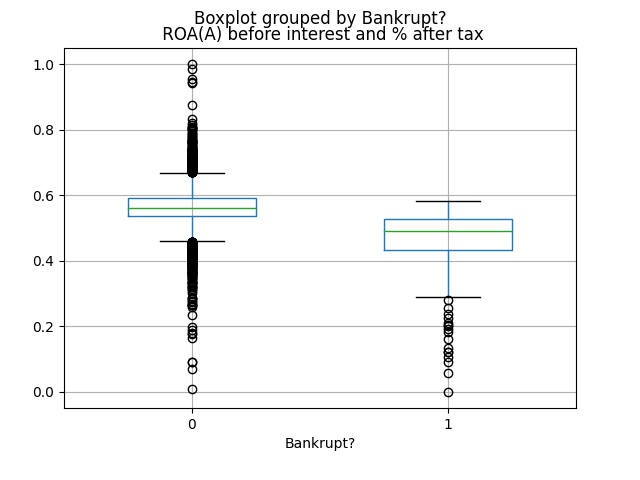
\includegraphics[height=1.8in]{figures/ ROA(A) before interest and after tax-boxplot.png}
      \caption{Box plot for attribute: Return on Assets}
  \end{subfigure}%
  ~ 
  \begin{subfigure}[t]{0.5\textwidth}
      \centering
      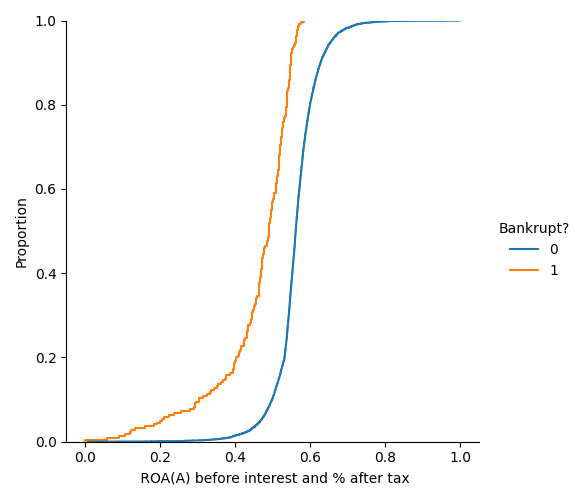
\includegraphics[height=1.8in]{figures/ ROA(A) before interest and after tax-displot.png}
      \caption{Distribution plot for attribute: Return on Assets}
  \end{subfigure}
  ~ 
  \begin{subfigure}[b]{0.5\textwidth}
      \centering
      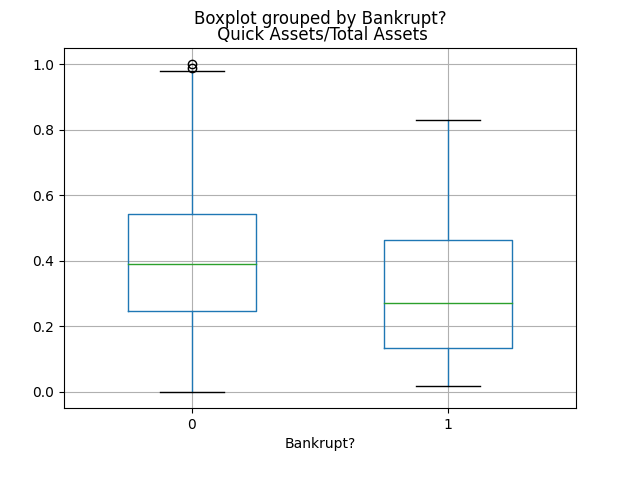
\includegraphics[height=1.8in]{figures/ Quick Assets_Total Assets-boxplot.png}
      \caption{Box plot for attribute: Quick Assets / Total Assets}
  \end{subfigure}%
  ~ 
  \begin{subfigure}[b]{0.5\textwidth}
      \centering
      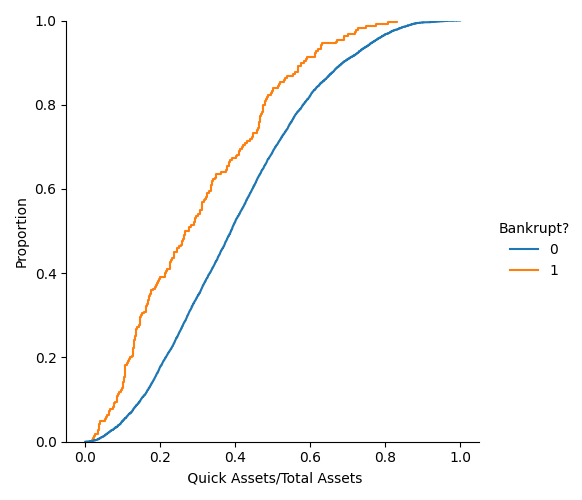
\includegraphics[height=1.8in]{figures/ Quick Assets_Total Assets-displot.png}
      \caption{Distribution plot for attribute: Quick Assets / Total Assets}
  \end{subfigure}
  \caption{Graphs from exploratory data analysis}
  \label{fig:eda}
\end{figure*}

\subsection{Exploratory Data Analysis}
\label{ssec:eda}

The first step to understanding data is exploratory data analysis. 
First we check for missing values and duplicates, which are not existent in our dataset.
Next we calculate the \emph{mean, standard deviation, minimum, maximum, Q1, median, Q3} for each attribute, the calculated values are in \ttt{project/exploratory-data-analysis/df-descrite.csv} in our GitHub repository.
To better visualize the data, we generated box plots and distribution plots for each attribute. 

As seen from the figures~\ref{fig:eda}, some attributes have different distributions when we group them by bankruptcy outcome.
From the graphs, we can infer that companies with lower \emph{ROA} and \emph{Quick Assets / Total Assets} ratios are more likely to go bankrupt.

We also analyzed the correlation between various attributes, which can be helpful for dimension reduction as we have 95 attributes.
The complete heatmap for correlation between the attributes is very large, therefore we did not include it in this report. 
The heatmap can be found in the file \ttt{project/exploratory-data-analysis/figures/heatmap.png} in our GitHub repository.
Attribute pairs such as \emph{(operating gross margin, realized sales gross margin)} or \emph{(pre-tax net interest rate, after-tax net interest rate)} have a correlation of nearly 1.

Additionally, we addressed class imbalance by calculating the frequency of each bankruptcy outcome, as displayed in Figure~\ref{fig:bankruptcy-outcome}. 
The severe data imbalance toward 'not bankrupt' highlights the necessity of implementing sampling methods, such as SMOTE~\cite{chawla2002smote}, to ensure balanced training data.

\begin{figure}
  \centering
  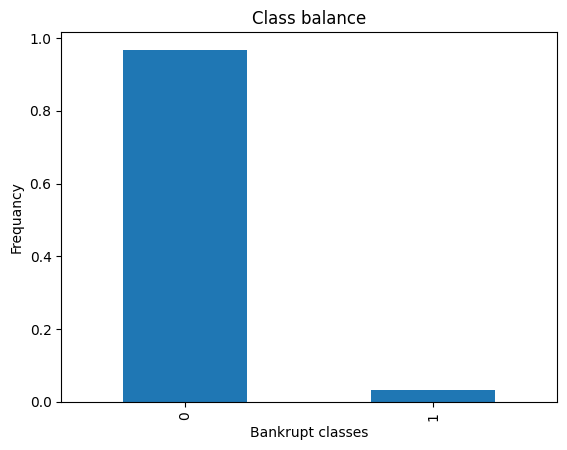
\includegraphics[height=2in]{figures/bankrupt-distribution.png}
  \caption{Relative frequency of bankruptcy outcome}
  \label{fig:bankruptcy-outcome}
\end{figure}


\subsection{Feature Selection}
\label{ssec:feature-selection}

We choose Mutual Information (MI) for feature selection in a dataset with 96 attributes to mitigate the curse of dimensionality. 
The \ttt{mutual\_info\_classif} function from scikit-learn was employed to compute feature scores, which measure the importance of each attribute in predicting the target feature. 
As shown in figure~\ref{fig:scree-plot}, a visual representation of these scores revealed that some attributes had very low scores, and a few even scored zero, indicating their limited contribution to the target prediction. 
To streamline the dataset and enhance model efficiency, a threshold of 0.005 was established, and attributes with scores below this value were removed. 
As a result, the initial set of 96 attributes was reduced to a more manageable 65, focusing on the most informative features for the predictive model.

\begin{figure}
  \centering
  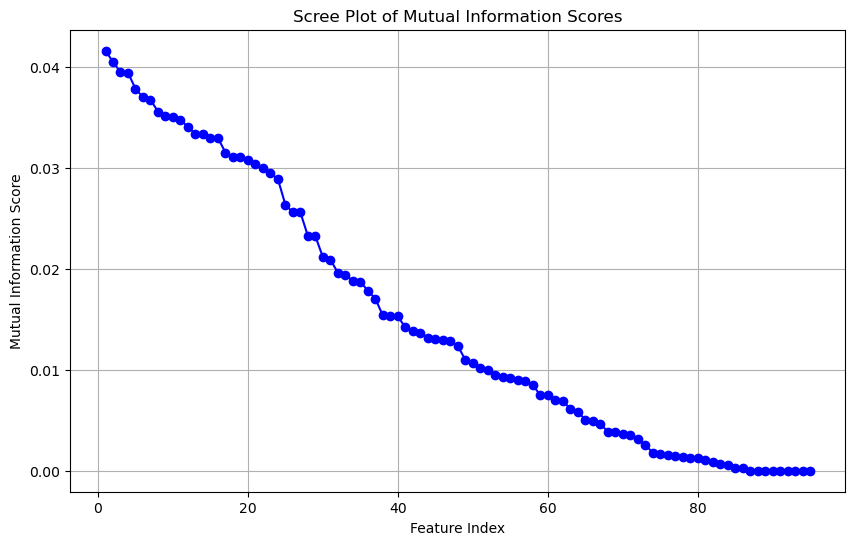
\includegraphics[height=3in]{figures/feature_scores.png}
  \caption{Scree plot of mutual information scores}
  \label{fig:scree-plot}
\end{figure}

\subsection{Resampling}
\label{ssec:resampling}

Through exploratory data analysis, we can see that there is a heavy class imbalance between the bankrupt data points and the not bankrupt data points. 
Of the 6819 records that we have, there are only 220 records for bankrupt companies whereas there are 6599 records for not bankrupt companies. 
Only 3.22\% of the total dataset contains records of bankrupt companies. 
Therefore, there is an inherent bias, where just predicting that a company will not go bankrupt will have an accuracy of 96.77\%.

Resampling methods such as \emph{RandomOverSampler, SMOTE, ADASYN,RandomUnderSampler, NearMiss}, and \emph{ClusterCentroids} were implemented in the code. 
SMOTE (Synthetic Minority Over-sampling Technique) was chosen as the initial resampling method because of its established effectiveness in generating synthetic examples for the minority class, addressing class imbalance, and improving the model's ability to handle imbalanced data. 

\subsection{Model Building and Cross Validation}
\label{ssec:model-cv}
To ensure a reliable evaluation, we implemented a 13-fold cross-validation strategy with data shuffling and a fixed random seed for reproducibility. This means our dataset is split into 13 subsets, and the model is trained and tested 13 times, ensuring thorough validation.
The \ttt{cross\_val\_predict} function is then employed to generate predictions for each data point in our dataset. 
This allows us to assess the model's performance more comprehensively, as we obtain predictions for all data points across multiple cross-validation folds.
The random forest classifier is used to predict the bankruptcy outcome.




\section{Preliminary Results}
\label{sec:results}

We ran our random forest classifier using 13-fold cross validation and achieved a f1-score of 0.98. Our results are shown in table~\ref{table:results}.

It can be concluded that the random forest classifier  has high precision and recall for both classes (0 and 1).
This indicates that the model is good at correctly identifying both classes with an overall high accuracy of 98\%. 
The f1-score, which combines precision and recall, is also high at 0.98, reflecting strong model performance. 
The macro and weighted averages of these metrics confirm the model's effectiveness in making accurate predictions for the dataset with balanced support for both classes.


\begin{table*}
  \caption{Preliminary results from running random forest classifier}
  \label{table:results}
  \centering
  
  \begin{tabular}{cccccc}
    \toprule
     & \textbf{Precision} & \textbf{Recall} & \textbf{f1-score} & \textbf{Support}  \\ 
    \midrule
    Bankruptcy = 0 & 1.00 & 0.96 & 0.98 & 6599 \\ 
    % \midrule
    Bankruptcy = 1 & 0.97 & 1.00 & 0.98 & 6599 \\
    % \hline
    accuracy & & & 0.98 & 13198\\
    % \hline
    macro avg & 0.98 & 0.98 & 0.98 & 13198\\ 
    % \hline
    weighted avg & 0.98 & 0.98 & 0.98 & 13198\\
    \bottomrule
  \end{tabular}
  \end{table*}


\section{Conclusion}
\label{sec:conclusion}

Thus far, we have applied sampling methods on the data and implemented it on a classifier. 
Between now and the final due date, we plan to apply other classifiers and methods and better understand what features contributed most.

Our future steps include:
\begin{enumerate}
  \item Applying various classification algorithms, including ensemble methods, and conducting hyperparameter tuning to enhance model performance.
  \item Assessing model performance using different implemented sampling techniques.
  \item Exploring additional feature selection and extraction techniques such as PCA to further optimize model performance.
  
\end{enumerate}


% \section{Conclusion}
% \label{sec:conclusion}


\bibliographystyle{plain}
\bibliography{references}

%%%%%%%%%%%%%%%%%%%%%%%%%%%%%%%%%%%%%%%%%%%%%%%%%%%%%%%%%%%%


\end{document}